% =============================================================================================
%  Multimodal Hateful Meme Detection: Does Fusion Beat Unimodal?
%  Overleaf: New Project -> Upload Project -> upload this file + the figures/ folder.
%  Compiler: pdfLaTeX. Every number comes from the results/ folder of the GitHub repository.
%  Section owners are marked with  % OWNER: <name>  -- read and edit your own sections.
% =============================================================================================
\documentclass[conference]{IEEEtran}
\usepackage[utf8]{inputenc}
\usepackage{amsmath,amssymb}
\usepackage{graphicx}
\usepackage{booktabs}
\usepackage{multirow}
\usepackage{xcolor}
\usepackage[hidelinks]{hyperref}
\graphicspath{{figures/}}
\newcommand{\best}[1]{\textbf{#1}}

\begin{document}

\title{Multimodal Hateful Meme Detection:\\ Does Fusion Beat Unimodal?}


\author{
\IEEEauthorblockN{Mohit Sharma, Yuvraj Chirag, Shlok Gupta, Ramraj Nagar}
\IEEEauthorblockA{Deep Learning (Semester 5), Sitare University\\
Code: \url{https://github.com/sharma-mohit-2005/hateful-memes-fusion}}
}

\maketitle

% OWNER: Mohit ------------------------------------------------------------------------------
\begin{abstract}
Hateful memes combine an image and a short caption whose meaning often emerges only from the two together; the
Hateful Memes Challenge makes this explicit through \emph{benign confounders}, near-duplicate memes whose label
flips when only the image or only the text is changed. We ask whether fusing the two modalities beats unimodal
models and which fusion strategy works best. We compare fine-tuned BERT and ResNet-50 baselines with early and late
fusion, and train eight fusion heads on frozen CLIP ViT-L/14 embeddings under an identical protocol (three seeds,
validation-based model selection). An element-wise product fusion of CLIP features reaches a test AUROC of
$0.826\pm0.002$, $+0.089$ over the best unimodal CLIP head and $+0.135$ over fine-tuned BERT. Fusion heads with an
explicit image--text interaction outperform concatenation, attention and late fusion. On 404 benign-confounder pairs
the best model ranks the hateful twin higher in 91\% of pairs, versus close to chance for text-only models. A
modality-shuffling test confirms that the model relies on both inputs, and removing the printed caption from the
images shows that much of CLIP's ``image-only'' performance comes from reading the text in the pixels (AUROC
$0.737\rightarrow0.634$). An error analysis attributes the remaining misses mainly to image--text interactions and
missing world knowledge.
\end{abstract}

\begin{IEEEkeywords}
multimodal learning, hateful memes, CLIP, fusion, benign confounders
\end{IEEEkeywords}

% OWNER: Mohit ------------------------------------------------------------------------------
\section{Introduction}
Memes are one of the main ways hate speech spreads online, and they are hard to moderate automatically: a caption
such as ``look how many people love you'' is harmless above a crowded stadium and hateful above an empty desert. The
Hateful Memes Challenge~\cite{kiela2020} was built to measure exactly this. Its \emph{benign confounders} are memes
that share the text (or the image) with a hateful meme but carry the opposite label, so neither a text-only nor an
image-only model can solve the task.

This project asks one main question: \emph{does fusion beat unimodal models, and which fusion strategy works best?}
We address five research questions:
\begin{enumerate}
  \item How much does fusing image and text improve over the best single modality?
  \item Which fusion operator works best on top of frozen CLIP embeddings?
  \item How do the models behave on benign-confounder pairs?
  \item Does the fused model really use both modalities?
  \item Is a CLIP ``image-only'' model really image-only, given that CLIP can read text in images?
\end{enumerate}

Our contributions are: (i) a controlled comparison of unimodal, early, late and eight intermediate fusion models,
all trained with the same protocol and three seeds; (ii) a benign-confounder analysis with a threshold-free
\emph{pair-rank} metric; (iii) a test-time modality-shuffling test; (iv) a caption-removal (inpainting) experiment
that isolates the visual signal; and (v) a manual error analysis of the best model. All code, predictions and
metrics are public in our repository.

% OWNER: Yuvraj -----------------------------------------------------------------------------
\section{Related Work}
\textbf{Hateful Memes.} Kiela et al.~\cite{kiela2020} released 10k+ memes built from licensed images with
re-written captions and benign confounders, and benchmarked unimodal models (image grid/region features, BERT),
simple fusion (late fusion, concatenation) and multimodally pre-trained transformers such as
ViLBERT~\cite{lu2019vilbert} and VisualBERT~\cite{li2019visualbert}. They reported that unimodal models perform
poorly, multimodal pre-training helps, and all models remain far below human accuracy (84.7\%).

\textbf{Pre-trained encoders.} BERT~\cite{devlin2019} and ResNet~\cite{he2016} are the standard text and image
encoders for fine-tuning. CLIP~\cite{radford2021} trains an image and a text encoder contrastively on 400M
image--caption pairs, so both modalities land in one shared embedding space; it is known to transfer well and to
read text rendered in images.

\textbf{Fusion of CLIP features.} Hate-CLIPper~\cite{kumar2022} trains small heads on frozen CLIP features and
shows that a \emph{feature interaction matrix} (outer product of projected image and text embeddings) is very
effective on Hateful Memes. Our ``cross'' operator follows this idea, and we compare it with simpler and more
complex alternatives under one protocol.

% OWNER: Shlok ------------------------------------------------------------------------------
\section{Dataset}
We use the Hateful Memes dataset~\cite{kiela2020}. Each sample is an image, its caption text and a binary label
(1 = hateful). We train on \texttt{train}, use \texttt{dev\_seen} as validation (\texttt{val}) for all model
selection and tuning, and report on \texttt{test\_seen} (\texttt{test}); \texttt{test\_unseen} is an additional
test set. Table~\ref{tab:data} summarises the splits.

\begin{table}[t]
\centering
\caption{Dataset splits (from \texttt{results/eda\_stats.csv}).}
\label{tab:data}
\begin{tabular}{lrrrr}
\toprule
Split & Memes & Hateful (\%) & Mean words & Max words \\
\midrule
train & 8{,}500 & 35.5 & 11.7 & 70 \\
val (dev\_seen) & 500 & 49.4 & 10.2 & 42 \\
test (test\_seen) & 1{,}000 & 49.0 & 10.4 & 57 \\
test\_unseen & 2{,}000 & 37.5 & 9.0 & 47 \\
\bottomrule
\end{tabular}
\end{table}

\begin{figure}[t]
\centering
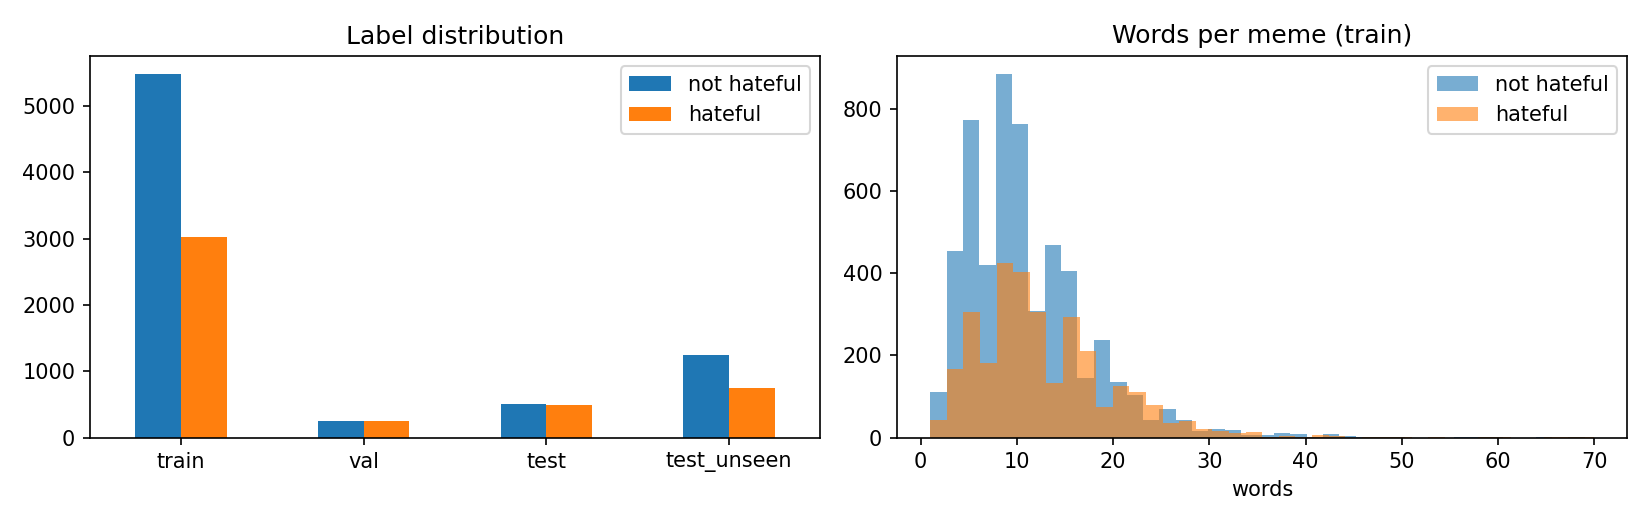
\includegraphics[width=\linewidth]{eda_distribution.png}
\caption{Label distribution per split (left) and caption length in the training set (right).}
\label{fig:eda}
\end{figure}

The training set is imbalanced (35.5\% hateful) while the evaluation splits are close to balanced
(Fig.~\ref{fig:eda}). We therefore use AUROC as the primary metric: it is threshold-independent and not affected by
the class ratio; accuracy and F1 at threshold 0.5 are reported as secondary metrics. Captions are short (11.7 words
on average), so a BERT maximum length of 64 tokens covers almost all of them. In the training set, 2{,}466 memes share
their exact caption with another meme and 636 captions appear with \emph{both} labels---the text-side benign
confounders that make text-only classification impossible for these memes.

\textbf{Data source.} The Hugging Face mirror we used (\texttt{neuralcatcher/hateful\_memes}) lacks 2{,}476 of the
12{,}140 images. Our download script fills these from a second mirror (\texttt{limjiayi/hateful\_memes\_expanded}),
taking only the images; the labels and splits are the original ones, so all 12{,}140 memes are complete and our
numbers are comparable with the original benchmark.

\section{Methods}
% OWNER: Yuvraj (A) + Shlok (B) -------------------------------------------------------------
\subsection{Fine-tuned baselines (M1--M4)}
\textbf{M1 (text only)} fine-tunes \texttt{bert-base-uncased}~\cite{devlin2019} and classifies the [CLS] vector.
\textbf{M2 (image only)} fine-tunes an ImageNet-pre-trained ResNet-50~\cite{he2016} (224$\times$224, random resized
crop, flip and colour jitter on train). \textbf{M3 (early fusion)} concatenates the BERT [CLS] vector (768-d) and the
pooled ResNet features (2048-d) and trains an MLP and both encoders end to end. \textbf{M4 (late fusion)} combines
the probabilities of M1 and M2, either averaged or as $w\,p_\text{text}+(1-w)\,p_\text{image}$ with $w$ chosen on
validation AUROC. All fine-tuned models use AdamW with differential learning rates (BERT $2\!\times\!10^{-5}$,
ResNet $10^{-4}$, head $10^{-3}$), linear warm-up and decay, mixed precision and gradient clipping; they train for
4/6/5 epochs (M1/M2/M3) with batch size 32 (16 for M3), keeping the epoch with the best validation AUROC.

% OWNER: Shlok (features) + Mohit (heads) ---------------------------------------------------
\subsection{Frozen CLIP features}
We encode every meme once with CLIP ViT-L/14~\cite{radford2021} and cache the projected image embedding
$\mathbf{x}_i$ and text embedding $\mathbf{x}_t$ (both 768-d; captions truncated to 77 tokens). CLIP stays frozen:
it is far larger than our 8.5k training memes justify fine-tuning, and caching makes every head train in seconds.
\textbf{M5} is a logistic-regression linear probe on the L2-normalised image, text or concatenated features, with the
regularisation strength chosen on validation (best $C=3$ in all three cases).

% OWNER: Mohit ------------------------------------------------------------------------------
\subsection{Fusion heads (M6, M7 and ablation)}
Each head L2-normalises both embeddings and projects them with separate layers
$\mathbf{i}=\mathrm{GELU}(W_i\hat{\mathbf{x}}_i)$, $\mathbf{t}=\mathrm{GELU}(W_t\hat{\mathbf{x}}_t)$ to $d=512$
(64 for \emph{cross}). A fusion operator produces $\mathbf{z}$, followed by a LayerNorm--MLP classifier
(512 hidden units, dropout 0.3) that outputs one logit. The operators are:
\begin{itemize}
  \item \emph{image\_only} / \emph{text\_only}: $\mathbf{z}=\mathbf{i}$ or $\mathbf{z}=\mathbf{t}$ (unimodal heads);
  \item \emph{concat} (M6): $\mathbf{z}=[\mathbf{i};\mathbf{t}]$;
  \item \emph{product}: $\mathbf{z}=\mathbf{i}\odot\mathbf{t}$;
  \item \emph{concat\_product}: $\mathbf{z}=[\mathbf{i};\mathbf{t};\mathbf{i}\odot\mathbf{t};|\mathbf{i}-\mathbf{t}|]$;
  \item \emph{cross} (M7, Hate-CLIPper style~\cite{kumar2022}): $\mathbf{z}=\mathrm{vec}(\mathbf{i}\,\mathbf{t}^{\top})$,
        a $64\times64$ interaction matrix;
  \item \emph{gated}: $\mathbf{g}=\sigma(W_g[\mathbf{i};\mathbf{t}])$, $\mathbf{z}=\mathbf{g}\odot\mathbf{i}+(1-\mathbf{g})\odot\mathbf{t}$;
  \item \emph{attention}: a 2-layer pre-norm Transformer over the tokens [CLS, $\mathbf{i}$, $\mathbf{t}$] with learned
        modality embeddings, $\mathbf{z}$ = output at CLS.
\end{itemize}
We also train \emph{concat} with \emph{modality dropout} (each training sample loses one modality with probability
0.3) and a CLIP late-fusion baseline that averages the probabilities of the two unimodal heads.

\textbf{Protocol.} Every head is trained with binary cross-entropy, AdamW (lr $10^{-4}$, weight decay $10^{-2}$),
cosine schedule, batch size 64, up to 40 epochs with early stopping (patience 8) on validation AUROC, for seeds 0, 1
and 2. We report mean $\pm$ standard deviation over the seeds; the test set is never used for any choice.

% OWNER: Ramraj -----------------------------------------------------------------------------
\subsection{Analysis methods}
\textbf{Benign-confounder pairs.} In the test set we pair memes with the same normalised caption but a different
image (\emph{text pairs}) and memes whose CLIP image embeddings of the caption-free (inpainted) images have cosine
similarity $\geq0.93$ but different captions (\emph{image pairs}); pairs with opposite labels are confounder pairs.
For each model we compute \emph{pair\_acc} (both memes classified correctly at 0.5) and \emph{pair\_rank} (the hateful
meme receives the strictly higher probability; ties count as failures, 0.5 = chance).

\textbf{Modality reliance.} For each trained CLIP head we replace one modality at test time, either by a random
permutation across memes (\emph{shuffle}, averaged over 5 permutations) or by the training-set mean embedding, and
measure the AUROC drop.

\textbf{Caption removal.} We detect the overlaid text with EasyOCR~\cite{easyocr}, dilate the detected boxes and fill
them with Telea inpainting~\cite{telea2004} (Fig.~\ref{fig:inpaint}), then re-extract CLIP image features and retrain
the \emph{image\_only}, \emph{concat} and \emph{cross} heads. The text input is unchanged.

\begin{figure}[t]
\centering
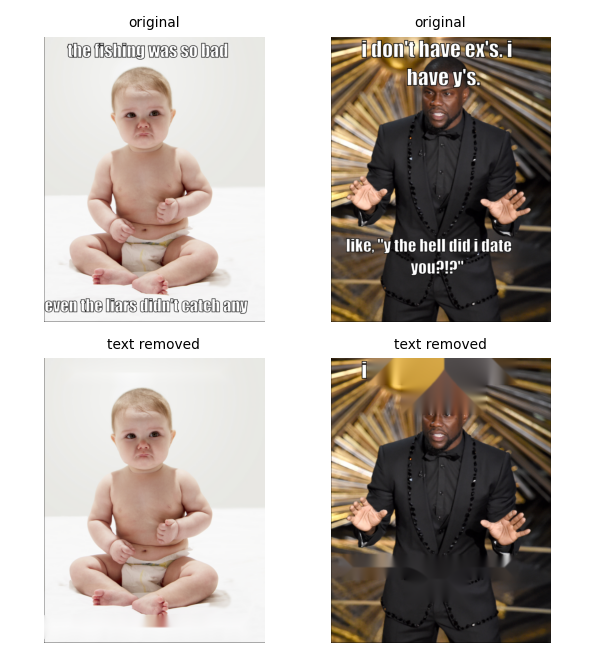
\includegraphics[width=0.75\linewidth]{inpaint_examples_safe.png}
\caption{Caption removal: original memes (top) and inpainted images (bottom). Small residues (e.g.\ the letter
``i'' on the right) and blurred regions remain.}
\label{fig:inpaint}
\end{figure}

% OWNER: Mohit ------------------------------------------------------------------------------
\section{Results}
Table~\ref{tab:main} and Fig.~\ref{fig:auroc} compare all models.

\begin{table}[t]
\centering
\caption{Main results (mean $\pm$ std over 3 seeds; linear probe: 1 deterministic run).}
\label{tab:main}
\setlength{\tabcolsep}{3pt}
\begin{tabular}{llccc}
\toprule
 & Model & Test AUROC & Test Acc & Unseen AUROC \\
\midrule
\multirow{4}{*}{\rotatebox{90}{\scriptsize Fine-tuned}}
 & M2 ResNet-50 (image) & $0.530\pm0.013$ & 0.509 & 0.548 \\
 & M1 BERT (text) & $0.691\pm0.005$ & 0.595 & 0.633 \\
 & M4 late fusion (weighted) & $0.693\pm0.004$ & 0.590 & 0.637 \\
 & M3 early fusion & $0.723\pm0.009$ & 0.626 & 0.685 \\
\midrule
\multirow{7}{*}{\rotatebox{90}{\scriptsize Frozen CLIP}}
 & text\_only head & $0.684\pm0.002$ & 0.608 & 0.630 \\
 & image\_only head & $0.737\pm0.002$ & 0.655 & 0.742 \\
 & M5 linear probe (concat) & $0.760$ & 0.669 & 0.740 \\
 & late fusion (average) & $0.759\pm0.002$ & 0.651 & 0.732 \\
 & M7 cross & $0.797\pm0.004$ & 0.721 & 0.785 \\
 & M6 concat & $0.799\pm0.002$ & 0.718 & 0.795 \\
 & product & \best{0.826}$\pm$\best{0.002} & \best{0.737} & \best{0.819} \\
\bottomrule
\end{tabular}
\end{table}

\begin{figure}[t]
\centering
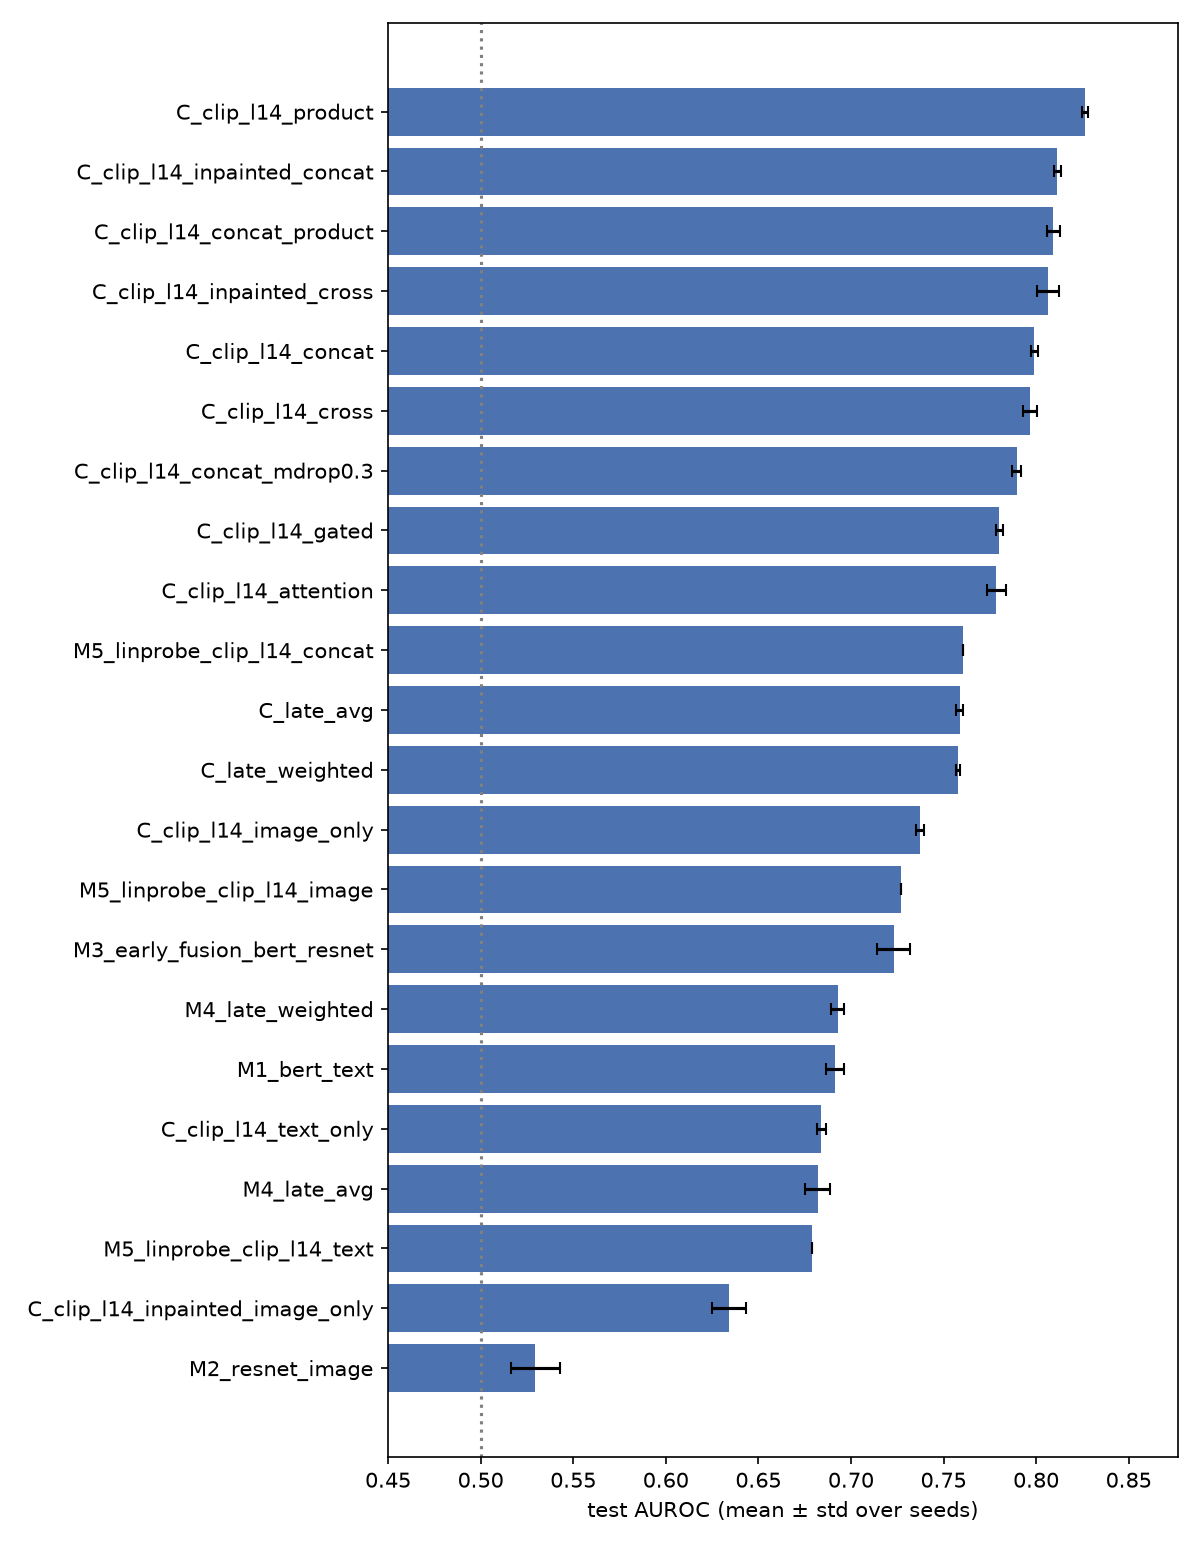
\includegraphics[width=\linewidth]{test_auroc.png}
\caption{Test AUROC of all 22 runs (error bars: std over seeds). \texttt{C\_clip\_l14\_*}: heads on frozen CLIP
features; \texttt{inpainted}: images with the caption removed.}
\label{fig:auroc}
\end{figure}

\textbf{RQ1: fusion beats unimodal.} With identical frozen CLIP features, the best fusion head improves over the best
unimodal head by $+0.089$ AUROC (0.826 vs.\ 0.737) and over the text head by $+0.142$; with fine-tuned encoders, early
fusion improves over BERT by $+0.032$. The conclusion holds on \texttt{test\_unseen} (0.819 vs.\ 0.742 for the best
unimodal head). Fusion therefore clearly beats unimodal models, but \emph{how} the modalities are fused matters: late
fusion gains little over the best unimodal model (0.693 vs.\ 0.691 with fine-tuned encoders, 0.759 vs.\ 0.737 with
CLIP, and on \texttt{test\_unseen} CLIP late fusion is even below the image head). Its weights also show which modality it
trusts: the tuned text weight is 0.75--0.95 for M4 (BERT is much stronger than ResNet) but 0.3 for CLIP, where the
image head is stronger.

\textbf{Features matter as much as fusion.} Every frozen-CLIP model that sees the image, from the image-only head
(0.737) and the linear probe (0.760) upwards, beats the fine-tuned BERT/ResNet early-fusion model (0.723). CLIP's jointly trained, aligned embedding space gives a much better starting
point on 8.5k training memes than two independently pre-trained encoders, and the ImageNet ResNet alone is close to
chance (0.530), in line with the weak image baselines reported in~\cite{kiela2020}.

\section{Fusion Ablation}
\begin{table}[t]
\centering
\caption{Fusion operators on frozen CLIP ViT-L/14 (test AUROC, mean $\pm$ std over 3 seeds).}
\label{tab:ablation}
\begin{tabular}{lcc}
\toprule
Operator & Test AUROC & Head params \\
\midrule
product $\mathbf{i}\odot\mathbf{t}$ & \best{0.826}$\pm$\best{0.002} & 1.05M \\
concat\_product & $0.809\pm0.004$ & 1.84M \\
concat (M6) & $0.799\pm0.002$ & 1.31M \\
cross (M7) & $0.797\pm0.004$ & 2.20M \\
concat + modality dropout & $0.790\pm0.002$ & 1.31M \\
gated & $0.780\pm0.002$ & 1.58M \\
attention & $0.779\pm0.005$ & 5.26M \\
late fusion (average) & $0.759\pm0.002$ & -- \\
\bottomrule
\end{tabular}
\end{table}

\textbf{RQ2.} Table~\ref{tab:ablation} shows that the simplest operator with an explicit image--text interaction, the
element-wise product, is the best and also one of the smallest heads. Adding the product and difference terms to the
concatenation (\emph{concat\_product}) improves over plain concatenation (0.809 vs.\ 0.799), so the gain comes from
the interaction terms, not from more capacity. The more expressive heads do not help: the attention head has five
times more parameters and is the weakest intermediate fusion, consistent with overfitting on 8.5k memes, and the
gated head, which mixes rather than multiplies the modalities, is similar. The outer-product \emph{cross} head did not
early-stop within 40 epochs for any seed and might improve with longer training. Modality dropout slightly hurts
(0.790 vs.\ 0.799) on this benchmark, where both modalities are always present at test time.

% OWNER: Ramraj -----------------------------------------------------------------------------
\section{Analysis}
\subsection{Benign confounders (RQ3)}
The test set contains 404 confounder pairs (174 text pairs, 230 image pairs). Table~\ref{tab:conf} reports the pair
metrics.

\begin{table}[t]
\centering
\caption{Benign-confounder pairs in the test set (mean over seeds).}
\label{tab:conf}
\begin{tabular}{lcc}
\toprule
Model & pair\_rank & pair\_acc \\
\midrule
M2 ResNet (image) & 0.471 & 0.039 \\
CLIP text\_only & 0.547 & 0.144 \\
M1 BERT (text) & 0.555 & 0.145 \\
CLIP image\_only & 0.706 & 0.341 \\
M3 early fusion & 0.740 & 0.289 \\
CLIP late fusion (avg.) & 0.809 & 0.283 \\
CLIP concat & 0.847 & 0.423 \\
CLIP product & \best{0.908} & \best{0.489} \\
\bottomrule
\end{tabular}
\end{table}

Text-only models are close to chance (pair\_rank $\approx$0.55): by construction they give the same score to both
memes of a text pair (a tie, counted as a failure), so they can only separate the image pairs, whose captions differ;
symmetrically, image-only models struggle on the near-identical image pairs. The fusion models separate the pairs
much better, and the best model ranks the hateful twin higher in 90.8\% of the pairs. Late fusion ranks pairs
reasonably (0.809) but rarely gets \emph{both} memes right (0.283), plausibly because averaging two unimodal opinions
cannot flip a decision that depends on their combination. Even the best model classifies both memes of a pair correctly in only
48.9\% of the pairs: it usually orders the pair correctly but places both on the same side of the 0.5 threshold,
in line with its tendency to under-predict hate (Section~\ref{sec:errors}).

\subsection{Modality reliance (RQ4)}
\begin{table}[t]
\centering
\caption{Test AUROC when one modality is shuffled or replaced by its training mean (mean over seeds).}
\label{tab:modality}
\setlength{\tabcolsep}{3pt}
\begin{tabular}{lccccc}
\toprule
Head & Original & Shuf.\ text & Shuf.\ image & Mean text & Mean image \\
\midrule
product & 0.826 & 0.630 & 0.601 & 0.707 & 0.666 \\
concat & 0.799 & 0.651 & 0.604 & 0.712 & 0.661 \\
cross & 0.797 & 0.623 & 0.594 & 0.701 & 0.657 \\
attention & 0.779 & 0.641 & 0.609 & 0.710 & 0.666 \\
concat (inpainted) & 0.811 & 0.568 & 0.625 & 0.633 & 0.669 \\
\bottomrule
\end{tabular}
\end{table}

Shuffling either modality causes a large drop for every fusion head (Table~\ref{tab:modality}), e.g.\ 0.826 to 0.630
(text) and 0.601 (image) for the product head, so the models genuinely use both inputs. Unimodal heads are unaffected
by shuffling the unused modality and fall to 0.50 when their own modality is shuffled, which validates the test.
Interestingly, once the caption is removed from the image, the fused model depends much more on the text channel
(shuffled text: 0.568 vs.\ 0.651), showing that with original images part of the caption information reaches the
model through the image encoder.

\subsection{Is CLIP image-only really image-only? (RQ5)}
\begin{table}[t]
\centering
\caption{Effect of removing the caption from the images (test AUROC).}
\label{tab:inpaint}
\begin{tabular}{lccc}
\toprule
Head & Original & Caption removed & $\Delta$ \\
\midrule
image\_only & 0.737 & 0.634 & $-0.103$ \\
concat & 0.799 & 0.812 & $+0.012$ \\
cross & 0.797 & 0.806 & $+0.010$ \\
\bottomrule
\end{tabular}
\end{table}

No. After removing the overlaid caption, the CLIP image-only head drops from 0.737 to 0.634
(Table~\ref{tab:inpaint}): a large part of its score came from CLIP \emph{reading} the caption in the pixels, which
also explains the gap to ResNet-50 (0.530). For the fusion heads the caption is already provided by the text encoder,
and removing it from the image slightly \emph{improves} AUROC, since the image embedding now describes only the
visual content and complements the text instead of duplicating it. The inpainting is imperfect (residual letters,
blurred patches, Fig.~\ref{fig:inpaint}), so the true image-only performance may be somewhat lower still.

% OWNER: Yuvraj -----------------------------------------------------------------------------
\section{Error Analysis}
\label{sec:errors}
Averaging the three seeds of the best model (product head), 264 of the 1{,}000 test memes are misclassified:
74 false positives (benign memes flagged as hateful) and 190 false negatives (hateful memes missed). The model
under-predicts hate, which is consistent with the shift from 35.5\% hateful memes in train to 49\% in test. We
manually categorised the 20 most confident errors of each kind after viewing each image together with its caption
(Table~\ref{tab:errors}).

\begin{table}[t]
\centering
\caption{Categories of the 20 most confident false positives (FP) and false negatives (FN) of the best model.}
\label{tab:errors}
\begin{tabular}{lccc}
\toprule
Category & FP & FN & Total \\
\midrule
image--text interaction & 3 & 10 & 13 \\
label noise & 8 & 1 & 9 \\
slur / keyword & 7 & 1 & 8 \\
world knowledge & 0 & 7 & 7 \\
other & 1 & 1 & 2 \\
sarcasm / irony & 1 & 0 & 1 \\
\midrule
Total & 20 & 20 & 40 \\
\bottomrule
\end{tabular}
\end{table}

The missed hateful memes mostly have a harmless caption whose meaning becomes hateful only with the specific image
(10), or require knowledge about a person, event or stereotype (7) that frozen CLIP features and a small head do not
capture. The confident false alarms are mostly memes that look hateful to a human annotator but are labelled benign
(8), or memes where the model reacts to an identity term or sensitive word although the image makes the meme harmless
(7)---exactly the dataset's benign confounders. Twelve of our 40 initial, text-only category assignments changed
after looking at the images, underlining that errors of a multimodal model have to be analysed multimodally.

% OWNER: Ramraj -----------------------------------------------------------------------------
\section{Limitations and Ethics}
\textbf{Limitations.} The training set is small (8.5k memes) and the labels are noisy, as our error analysis shows;
results on 1{,}000 test memes have non-negligible variance. We keep CLIP frozen and train small heads only, so we do
not test end-to-end fine-tuning or large vision--language models. Hyper-parameters were shared across heads rather
than tuned per head, and the \emph{cross} head may be under-trained. Confounder pairs are found automatically with a
similarity threshold and may contain a few non-pairs. The inpainting leaves residual text. The dataset is English-only
and US-centric.

\textbf{Ethics.} The dataset contains highly offensive content targeting protected groups; we never show raw hateful
memes in this report or commit meme images to the repository. A deployed detector would make errors in both
directions---missed hate harms targeted communities, false alarms censor legitimate speech---and our model
under-predicts hate, so it should only assist human moderators. Models trained on such data can learn spurious
associations between identity terms and hate (our ``slur / keyword'' errors), which could unfairly flag benign
content about these groups. The data is used under Meta's research licence and is not redistributed.

% OWNER: Mohit ------------------------------------------------------------------------------
\section{Conclusion}
Fusion clearly beats unimodal models on Hateful Memes: on the same frozen CLIP features, a simple element-wise
product of the image and text embeddings improves test AUROC from 0.737 to 0.826, ranks the hateful twin higher in
91\% of benign-confounder pairs, and relies on both modalities. The way the modalities are fused matters more than the
size of the head: explicit interactions beat concatenation, attention and late fusion. We also show that a CLIP
``image-only'' model largely reads the caption from the image. The remaining errors point to two directions for
future work: models with more world knowledge (e.g.\ large vision--language models) and better handling of label
noise and class imbalance (e.g.\ threshold calibration on validation).

\section*{Team Contributions}
\noindent\textbf{Mohit Sharma} (lead): designed the CLIP fusion study and implemented the fusion heads, training
script and linear probe (best model); found and fixed the missing-image problem in the dataset pipeline; produced
the final results tables, chart and README; maintained the Colab notebook; reviewed and merged all pull requests
and integrated the report.
\textbf{Yuvraj Chirag}: fine-tuned BERT/ResNet baselines, late fusion, error analysis.
\textbf{Shlok Gupta}: data pipeline and splits, exploratory data analysis, early fusion, CLIP feature extraction.
\textbf{Ramraj Nagar}: benign-confounder analysis, modality reliance test, caption-removal experiment.
Each member opened their own pull requests; the history is public in the repository.
Code scaffolding and parts of the documentation were assisted by an AI coding tool, as permitted for this course;
all experiments were run and checked by the team.

\begin{thebibliography}{9}
\bibitem{kiela2020} D.~Kiela, H.~Firooz, A.~Mohan, V.~Goswami, A.~Singh, P.~Ringshia, and D.~Testuggine, ``The Hateful
Memes Challenge: Detecting hate speech in multimodal memes,'' in \emph{NeurIPS}, 2020. arXiv:2005.04790.
\bibitem{radford2021} A.~Radford \emph{et al.}, ``Learning transferable visual models from natural language
supervision,'' in \emph{ICML}, 2021. arXiv:2103.00020.
\bibitem{kumar2022} G.~K.~Kumar and K.~Nandakumar, ``Hate-CLIPper: Multimodal hateful meme classification based on
cross-modal interaction of CLIP features,'' 2022. arXiv:2210.05916.
\bibitem{devlin2019} J.~Devlin, M.-W.~Chang, K.~Lee, and K.~Toutanova, ``BERT: Pre-training of deep bidirectional
transformers for language understanding,'' in \emph{NAACL}, 2019.
\bibitem{he2016} K.~He, X.~Zhang, S.~Ren, and J.~Sun, ``Deep residual learning for image recognition,'' in
\emph{CVPR}, 2016.
\bibitem{lu2019vilbert} J.~Lu, D.~Batra, D.~Parikh, and S.~Lee, ``ViLBERT: Pretraining task-agnostic visiolinguistic
representations for vision-and-language tasks,'' in \emph{NeurIPS}, 2019.
\bibitem{li2019visualbert} L.~H.~Li, M.~Yatskar, D.~Yin, C.-J.~Hsieh, and K.-W.~Chang, ``VisualBERT: A simple and
performant baseline for vision and language,'' 2019. arXiv:1908.03557.
\bibitem{telea2004} A.~Telea, ``An image inpainting technique based on the fast marching method,'' \emph{Journal of
Graphics Tools}, vol.~9, no.~1, 2004.
\bibitem{easyocr} JaidedAI, ``EasyOCR,'' \url{https://github.com/JaidedAI/EasyOCR}.
\end{thebibliography}

\end{document}
